\documentclass[11pt,a4paper]{article}

\usepackage[a4paper, portrait, margin=1.1in]{geometry}
\usepackage[dvipsnames]{xcolor}
\usepackage[linktoc=none]{hyperref}
\hypersetup{
	colorlinks=true,
	linkcolor=blue,
	filecolor=magenta,      
	urlcolor=blue,
}

\usepackage{listings}
\usepackage{float}
\usepackage{graphicx}
\usepackage[justification=centering]{caption}
\usepackage{wrapfig}
\usepackage{amsmath}

\renewcommand{\contentsname}{Indice}

\definecolor{anti-flashwhite}{rgb}{0.95, 0.95, 0.96}

\begin{document}

\begin{center}
	\Large\textbf{Classificazione dei Supercomputer}\\
	\vspace{0.2cm}
	\large{Progetto per il corso di Statistica del Prof. Marco Romito}\\
	\vspace{0.5cm}
	\large\textit{Rambod Rahmani}\\
	\vspace{0.2cm}
	\scriptsize{Corso di Laurea Magistrale in\\Artificial Intelligence and
	Data Engineering}\\
	\vspace{0.5cm}
	\normalsize{13 Dicembre 2020}
\end{center}

\tableofcontents

\section{Introduzione}
Lo scopo della presente analisi \`e quello di costruire un modello di
classificazione per poter determinare il segmento di mercato di appartenenza di
una Supercomputer a partire dalle specifiche delle sue caratteristiche hardware
e dalle prestazioni ottenute nei principali benchmarks utilizzati in questo
settore.
A partire dalla tabella dei dati, tramite l'utilizzo di R, a seguito di una
preliminare analisi delle componenti principali, sono stati valutati un modello
di classificazione mediante analisi discriminante lineare, uno mediante analisi
discriminante quadratica e uno di classificazione con la regressione
logistica.\\
\\
Per quanto riguarda il contesto applicativo ipotizzato, possiamo immaginarci che
un tale modello di classificazione possa essere utilizzato, al momento
dell'installazione di un nuovo Supercomputer, per individuare la fascia di
mercato pi\`u idonea in base alle sue prestazioni.

\section{Dati}
La tabella dei dati \`e stata scaricata dal sito dell'organizzazione
\textbf{TOP500}. La TOP500 mantiene una graduatoria, ordinata secondo le loro
prestazioni, dei Supercomputer attualmente installati e in funzione. Tale
graduatoria viene aggiornata con cadenza semestrale.\\
\textbf{Link di download diretto:} \url{https://www.top500.org/lists/top500/2020/11/download/TOP500_202011.xlsx}\\
\begin{figure}[h]
	\vspace{-1cm}
	\begin{minipage}{.3\textwidth}
		\textbf{Credenziali di accesso:}
	\end{minipage}
	\begin{minipage}{0.7\textwidth} 
		\begin{lstlisting}[language=bash,tabsize=2,backgroundcolor=\color{Goldenrod}]
		Login: rambodrahmani@yahoo.it
		Password: GCgFH6yuZYFMeCr
		\end{lstlisting}
	\end{minipage}
	\vspace{-1cm}
\end{figure}
\subsection{Contenuto della tabella}
La tabella dei dati contiene $37$ colonne per un totale di $500$ osservazioni.
Per la presente analisi ho utilizzato le seguenti colonne: \textbf{Site},
\textbf{Manufacturer}, \textbf{Country}, \textbf{Year}, \textbf{Segment},
\textbf{TotalCores}, \textbf{Rmax}, \textbf{Rpeak}, \textbf{Nmax},
\textbf{HPCG}, \textbf{Architecture}, \textbf{Processor},
\textbf{ProcessorTechnology}, \textbf{ProcessorSpeed}, \textbf{OperatingSystem},
\textbf{CoProcessor}, \textbf{CoresPerSocket}, \textbf{ProcessorGeneration},
\textbf{SystemModel}, \textbf{SystemFamily}, \textbf{InterconnectFamily},
\textbf{Interconnect}, \textbf{Continent}. Molti di questi fattori sono di tipo
categorico, quindi sono stati convertiti in numerici per non perdere
l'informazione in essi contenuta. A parte le colonne di significato ovvio, penso
sia doveroso fornire maggiori informazioni riguardo i seguenti fattori:
\begin{itemize}
	\setlength\itemsep{0mm}
	\item \textbf{Rmax [TFlop/s]}: massime prestazioni raggiunte nel
		benchmark LINPACK;
	\item \textbf{Rpeak [TFlop/s]}: massime prestazioni teoriche;
	\item \textbf{Nmax}: dimensione del problema sul quale \`e stato
		raggiunto il punteggio Rmax.
	\item \textbf{HPCG [TFlop/s]}: massime prestazioni raggiunte nel
		benchmark HPCG (High Performance Conjugate Gradient);
\end{itemize}
\subsection{Importazione e pulizia}
Sui dati, non \`e stata effettuata alcuna operazione precedente la loro
importazione in R. Il file originale, in formato \texttt{.xlsx}, \`e stato
per\`o convertito in \texttt{.csv} per facilitare l'importazione.\\
Prima di iniziare l'analisi, ho rimosso le colonne che ritengo non influenzino
la classificazione del segmento di mercato di un Supercomputer oppure con valore
costante per tutte le osservazioni (Rank TOP500, "Name", "Computer",
"Power.Source", "OS.Family", ecc\dots), mentre come fattore di uscita per la
classificazione \`e stato utilizzato il valore della colonna "\textbf{Segment}".
\begin{lstlisting}[language=bash,basicstyle=\footnotesize,tabsize=2,frame = single]
> with(data, table(Segment))
Segment
  Academic Government   Industry     Others   Research     Vendor 
        67         34        273         14        103          9
\end{lstlisting}
Nelle colonne che ho scelto, ho rilevato $351$ valori mancanti in
"Accelerator/Co-Processor Cores", $426$ in "HPCG [TFlop/s]" e $488$ in
"Nhalf". Dato che il numero di valori mancanti \`e elevato rispetto al
totale delle $500$ osservazioni, le suddette colonne sono state eliminate.

\section{Analisi}
Subito dopo l'importazione e la pulizia dei dati, sono state effettuate due
preliminari classificazioni ottenendo i seguenti risultati:
\begin{itemize}
	\item \textbf{Analisi Discriminante Lineare}: un'accuratezza non
		soddisfacente del $73.33\%$
	\begin{lstlisting}[language=bash,basicstyle=\scriptsize,tabsize=2,frame = single]
Confusion Matrix and Statistics

              Reference
Prediction    Academic  Government  Industry  Others  Research  Vendor
  Academic          42           2         8       0        22       2
  Government         4          16         1       0         2       0
  Industry           5           6       245      11        17       0
  Others             0           0         7       2         1       0
  Research          15          10         8       1        53       1
  Vendor             1           0         4       0         4       5

Overall Statistics
               Accuracy : 0.7333
	\end{lstlisting}
	\item \textbf{Analisi Discriminante Quadratica}: stiamo utilizzando $22$
		fattori con un numero di osservazioni pari a $495$
	\begin{lstlisting}[language=bash,basicstyle=\scriptsize,tabsize=2,frame = single]
Error in qda.default(x, grouping, ...) : 
  some group is too small for 'qda'
	\end{lstlisting}
\end{itemize}
Non \`e stata effettuata alcuna suddivisione dei dati in training set e test
set, e si ottengono risultati con capacit\`a predittiva inferiore all'$80\%$:
una analisi delle componenti principali per ridurre la dimensione del problema
si rivela quindi inevitabile.
\subsection{Preliminare analisi delle Componenti Principali}
Una prima analisi delle componenti principali, \textbf{non prendendo in
considerazione la classe delle osservazioni}, nonostante ci permetta di ridurre
il numero di fattori presi in considerazione, \textbf{porta a risultati persino
peggiori}: l'accuratezza della classificazione per mezzo di LDA scende al
$68\%$. Ho quindi valutato un secondo modello di PCA dove ho preso in
considerazione anche la classe delle osservazioni.
\begin{figure}[H]
	\hspace{-3.40cm}
	\begin{minipage}{0.73\textwidth}
		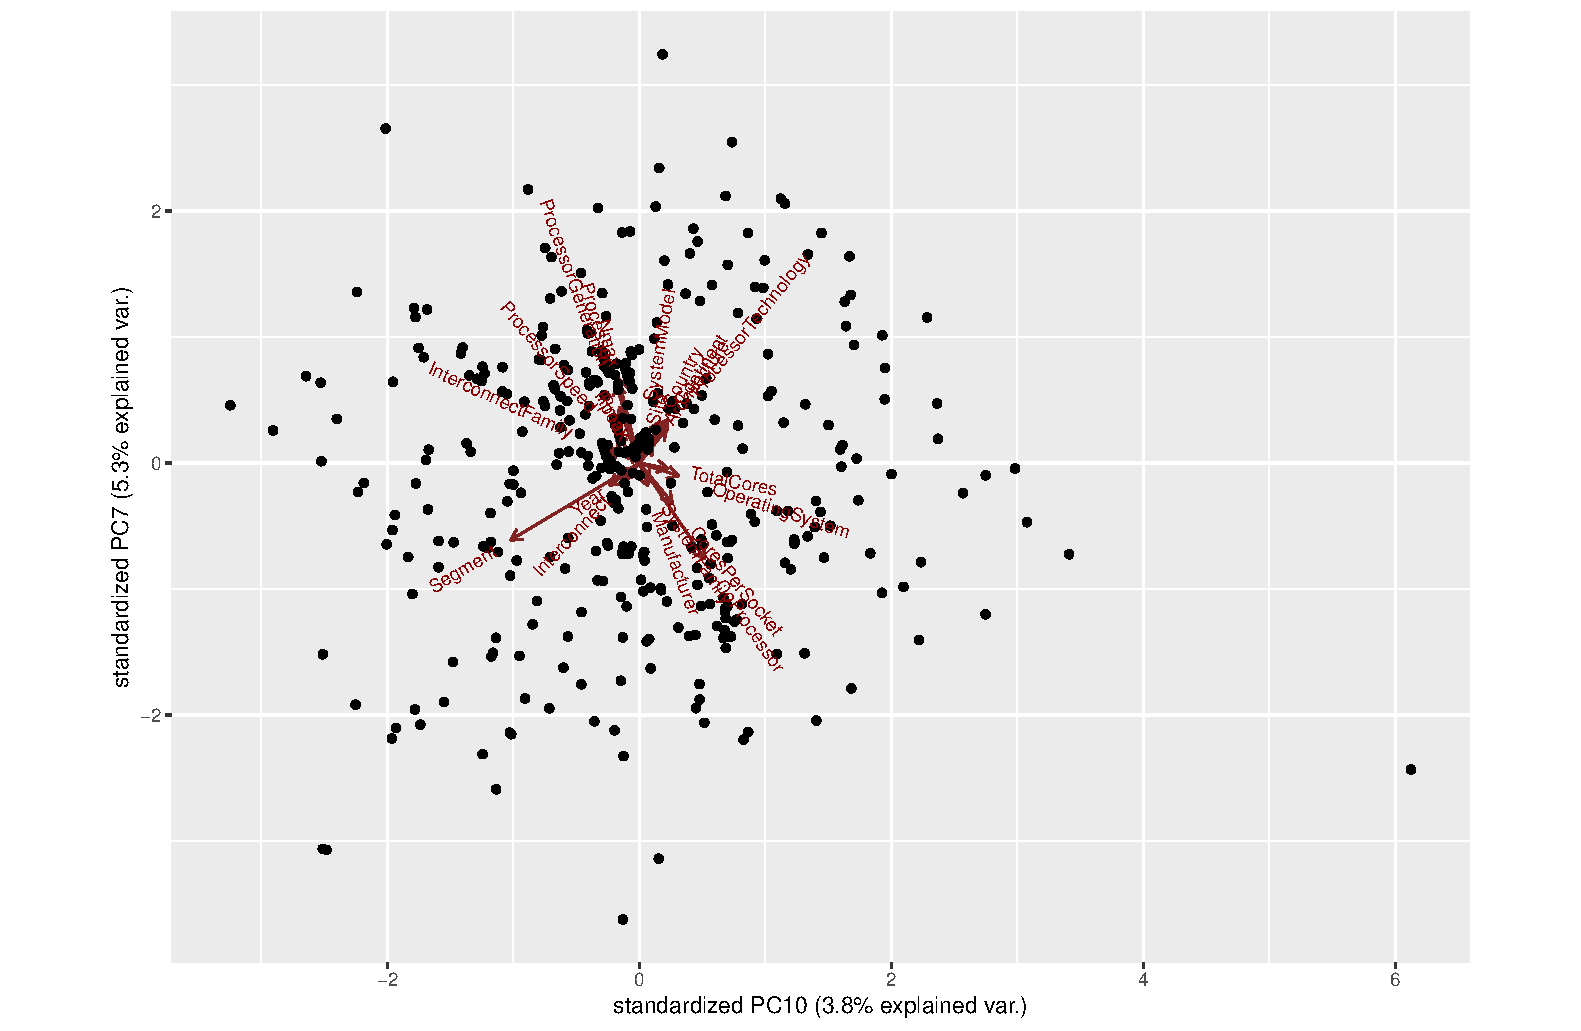
\includegraphics[scale=.45]{imgs/ggbiplot.pdf}
	\end{minipage}
	\begin{minipage}{0.5\textwidth}
		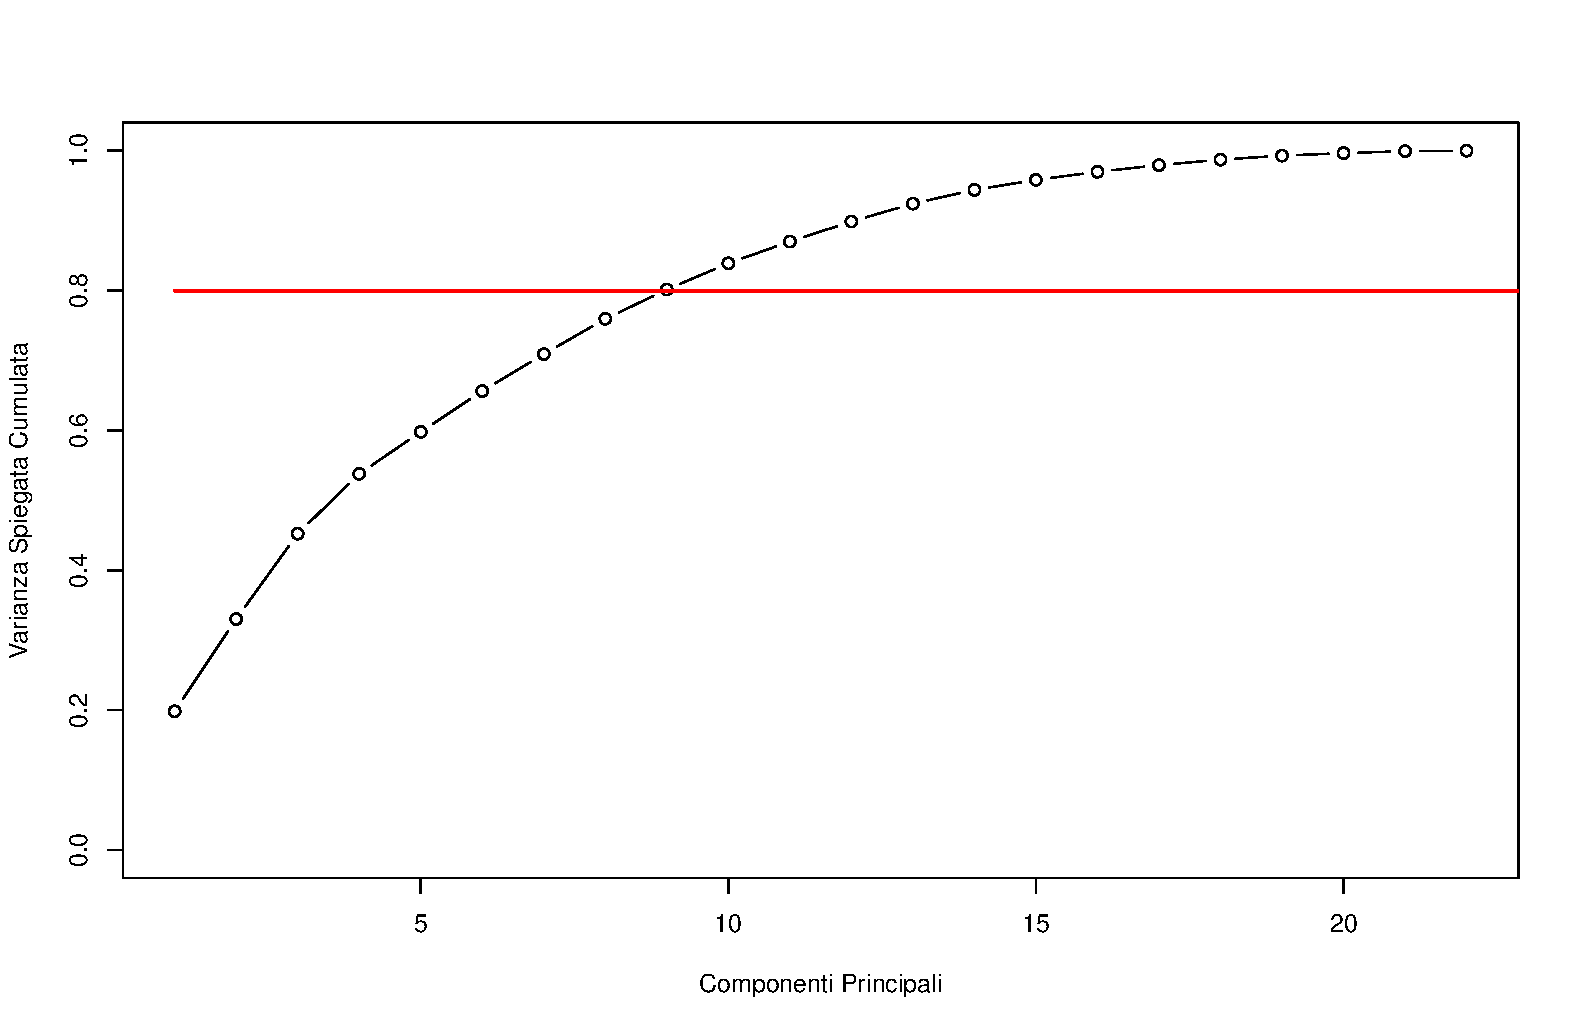
\includegraphics[scale=.38]{imgs/cumulative_variance.pdf}
	\end{minipage}
\end{figure}
\noindent Nonostante non si tratti certamente di un problema che potremmo
definire "passibile di riduzione", possiamo notare che con un numero di fattori
pari a $10$ catturiamo circa l'$85\%$ della struttura. Meno della met\`a quindi
del numero di fattori iniziali. \`E certamente un miglioramento. Ho identificato
le componenti principali che meglio catturavano la varianza del fattore
originario "Segment" analizzando gli allineamenti nel \textbf{biplot} e i
coefficienti della \textbf{matrice dei loading}. Con questo nuovo insieme di
fattori, \textbf{la dimensione di analisi del problema \`e diminuita
dall'iniziale $22$ a $5$}. Sono quindi stati valutati a questo punto un modello
di classificazione per mezzo di Analisi Discriminante Lineare, uno di
classificazione per mezzo di Analisi Discriminante Quadratica e uno di
classificazione per mezzo di Regressione Logistica. I risultati ottenuti sono
esposti nelle sezioni a seguire.
\subsection{Classificazione per mezzo di Analisi Discriminante Lineare}
Sono state utilizzate $5$ componenti principali ottenendo un'accuratezza media
dell'$85.55\%$ e una deviazione standard del $6.57\%$. Per ottenere risultati
statisticamente significativi l'esperimento \`e stato ripetuto $30$. Notiamo
quindi un netto miglioramento rispetto all'analisi preliminare precedente la
PCA.
\begin{figure}[H]
	\vspace{-2.5cm}
	\hspace{-0.8cm}
	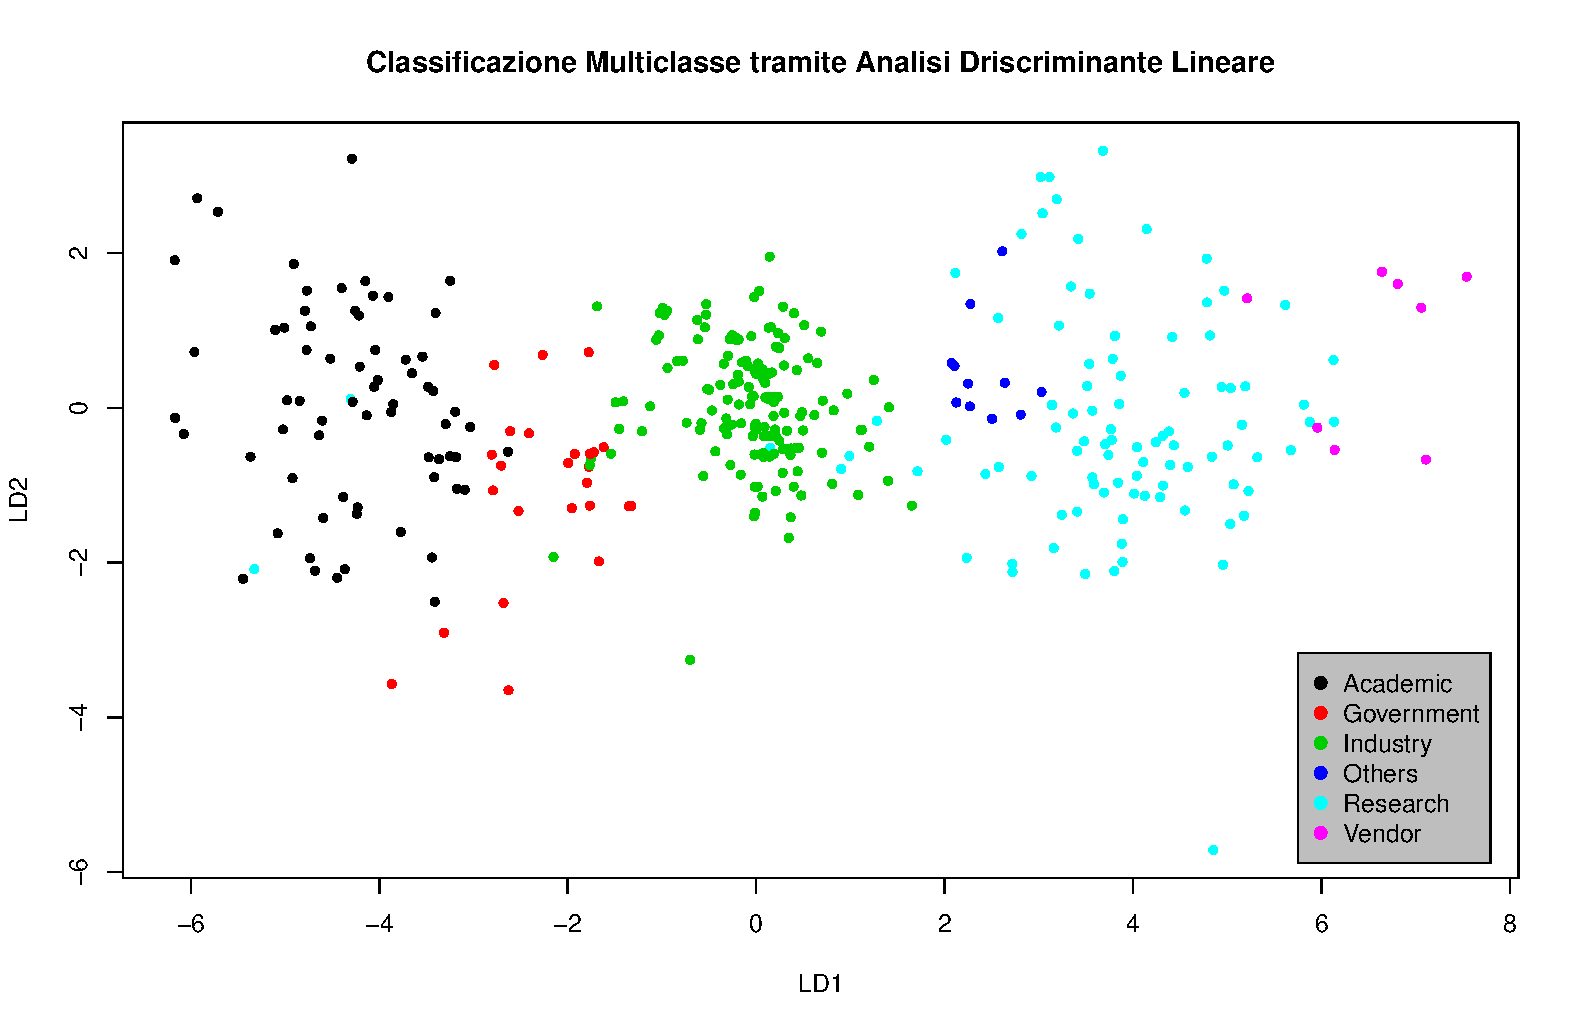
\includegraphics[scale=.59]{imgs/LDA_plot.pdf}
\end{figure}
\vspace{-0.6cm}
\begin{lstlisting}[language=bash,basicstyle=\scriptsize,tabsize=2,frame = single]
> confusionMatrix(as.factor(lda.values$class), as.factor(Segments))
Confusion Matrix and Statistics

             Reference
Prediction    Academic  Government  Industry  Others  Research  Vendor
  Academic          65           4         0       0         2       0
  Government         2           9         2       0         0       0
  Industry           0          21       271       0         6       0
  Others             0           0         0       8         6       0
  Research           0           0         0       6        82       1
  Vendor             0           0         0       0         3       7
Overall Statistics
               Accuracy : 0.8929          
\end{lstlisting}
\begin{figure}[H]
	\vspace{-0.1cm}
	\hspace{-0.9cm}
	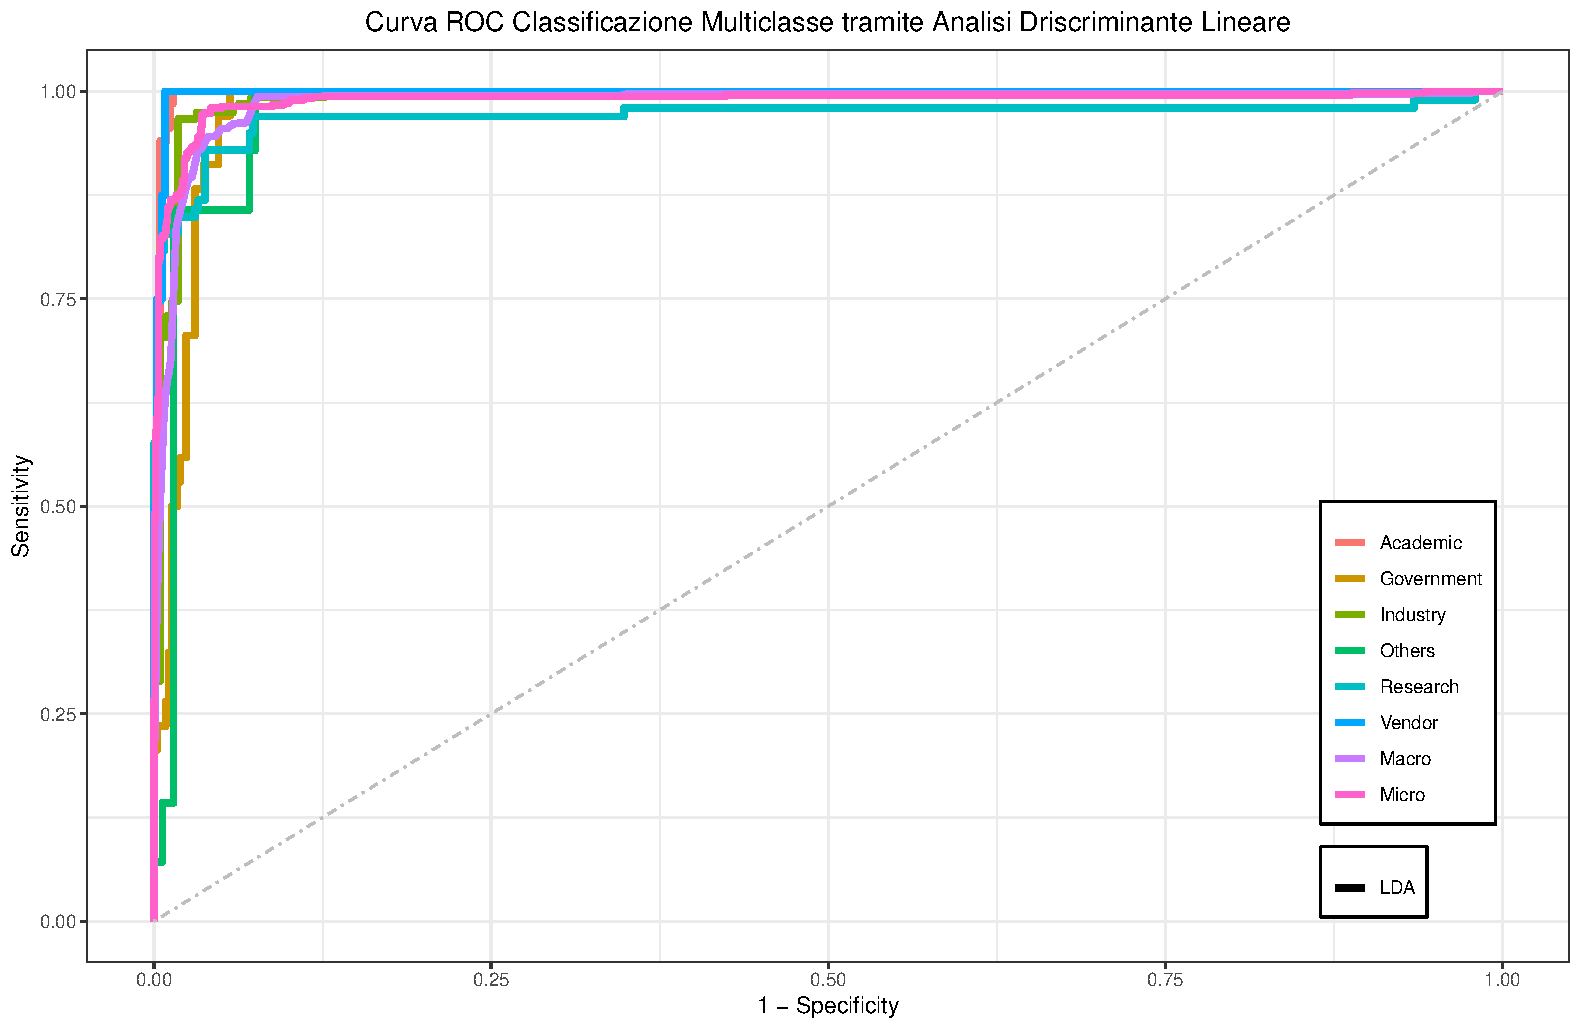
\includegraphics[scale=.59]{imgs/LDA_ggplot.pdf}
\end{figure}
\noindent I valori AUC: Area Under the ROC Curve per ogni classe sono i seguenti
\clearpage
-
\vspace{-1.22cm}
\begin{lstlisting}[language=bash,basicstyle=\scriptsize,tabsize=2,frame = single]
 Academic   Government   Industry   Others     Research   Vendor
 0.9968615  0.9812428    0.9912220  0.9787645  0.9700541  0.9976899
\end{lstlisting}
Non ci dobbiamo scordare che questi dati sono relativi all'utilizzo del modello
sugli stessi dati utilizzati per allenarlo. In fase di autovalutazione i valori
sono inferiori ovviamente:
\begin{figure}[H]
	\vspace{-0.5cm}
	\hspace{-0.9cm}
	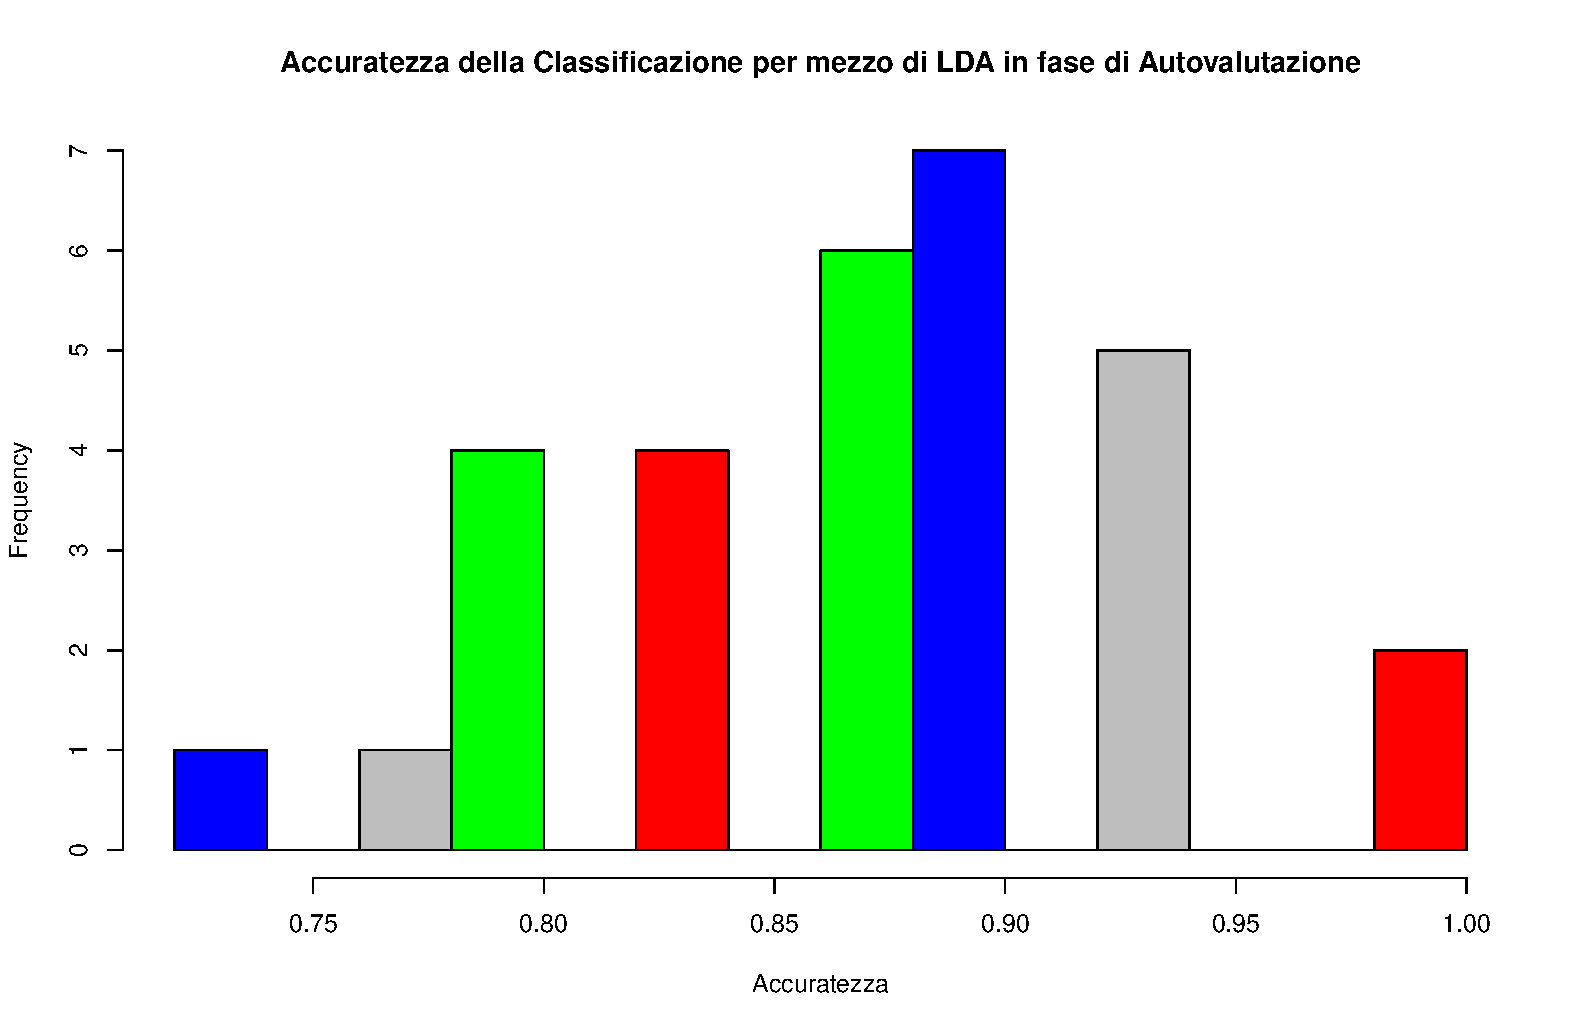
\includegraphics[scale=.58]{imgs/LDA_hist.pdf}
\end{figure}
\subsection{Classificazione per mezzo di Analisi Discriminante Quadratica}
Nell'analisi preliminare precedente alla PCA, non era stato possibile in alcun
modo costruire un modello di Classificazione Multiclasse per mezzo di Analisi
Discriminanete Quadratica dato che il numero di fattori era eccessivo rispetto
al numero totale di osservazioni, e a causa di collinearit\`a tra i fattori che
rendevano la matrice di Covarianza associata alla tabella singolare, non
invertibile.\\
\\
Grazie alla riduzione dimensionale del problema invece, utilizzando anche questa
volta $5$ componenti principali, si ottiene un modello di classificazione
multiclasse con un'accuratezza media dell'$88.33\%$ e una deviazione standard
del $5.85\%$. Per ottenere risultati statisticamente significativi l'esperimento
\`e stato ripetuto $30$ volte.
\begin{lstlisting}[language=bash,basicstyle=\scriptsize,tabsize=2,frame = single]
> confusionMatrix(as.factor(qda.values$class), as.factor(Segments))
Confusion Matrix and Statistics

             Reference
Prediction    Academic  Government  Industry  Others  Research  Vendor
  Academic          64           3         0       0         0       0
  Government         3          21         1       0         0       0
  Industry           0          10       262       0         1       0
  Others             0           0         0      12         1       0
  Research           0           0        10       2        94       3
  Vendor             0           0         0       0         3       5
Overall Statistics
               Accuracy : 0.9253
\end{lstlisting}
Raggiungiamo quindi un capacit\`a predittiva maggiore rispetto alla
classificazione per mezzo LDA. Utilizzando $5$ fattori con un totale di $500$
osservazioni inoltre, possiamo affermare che l'analisi non \`e affetta da
overfitting.
\clearpage
\begin{figure}[H]
	\vspace{-2.0cm}
	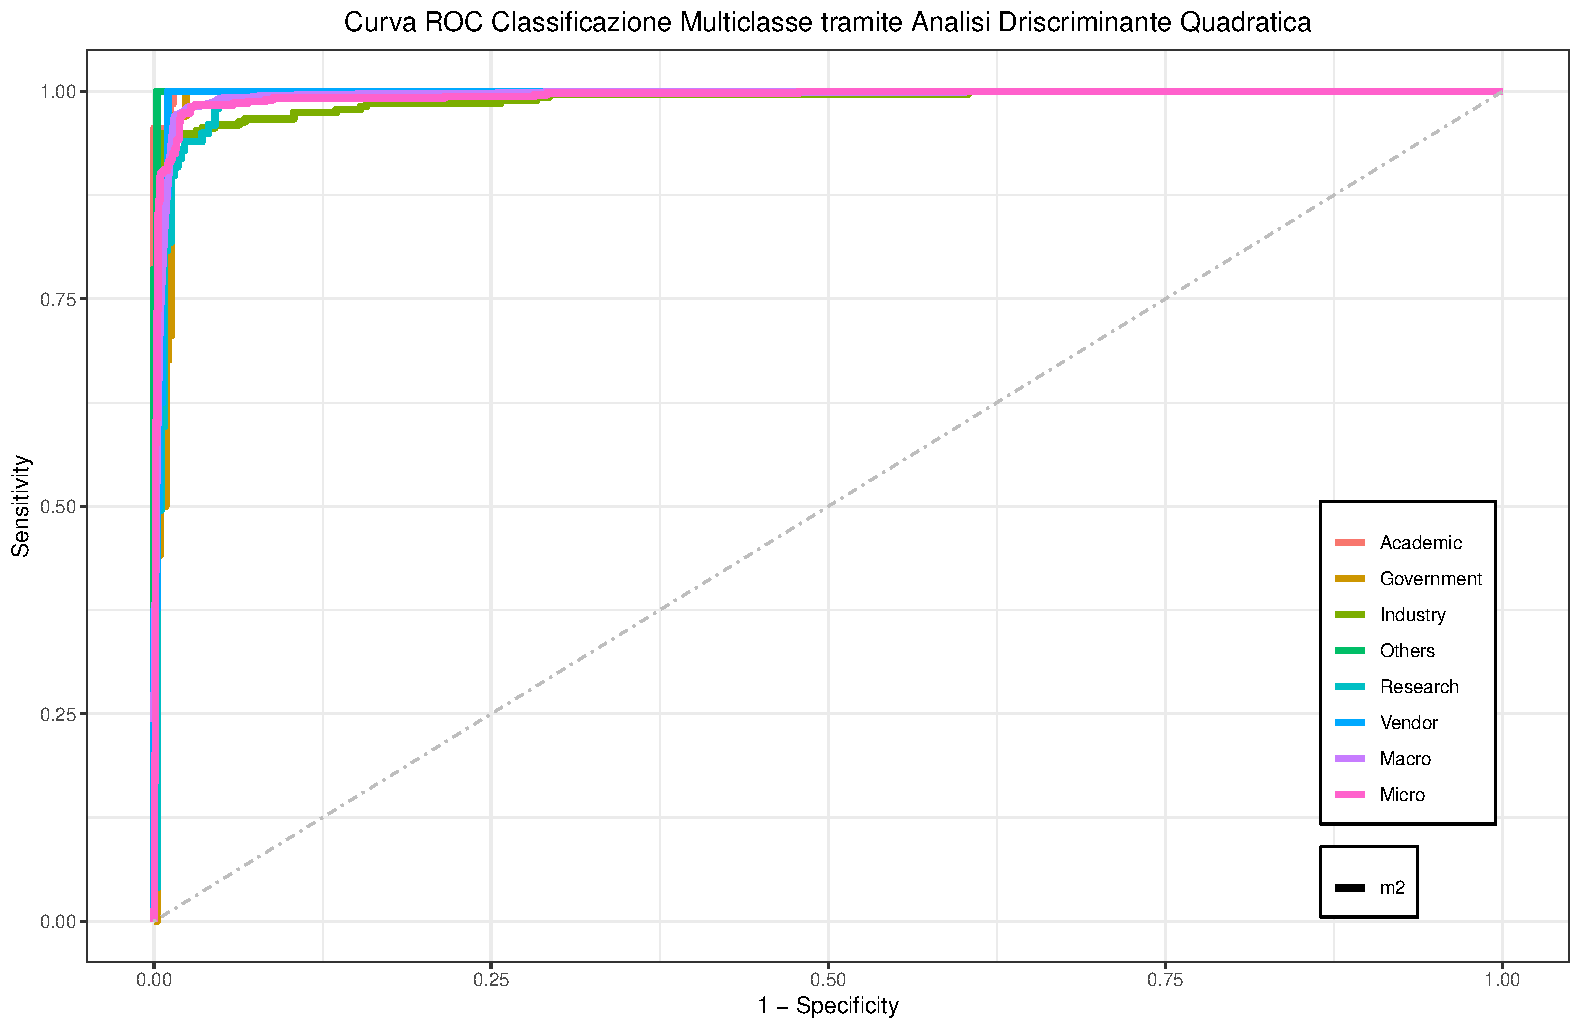
\includegraphics[scale=.55]{imgs/QDA_ggplot.pdf}
	\vspace{-0.4cm}
\end{figure}
\noindent I valori AUC: Area Under the ROC Curve per ogni classe sono i seguenti
\begin{lstlisting}[language=bash,basicstyle=\scriptsize,tabsize=2,frame = single]
 Academic   Government  Industry   Others     Research   Vendor
 0.9994420  0.9927906   0.9904795  0.9995545  0.9919141  0.9964066
\end{lstlisting}
In fase di autovalutazione la precisione di predizione \`e inferiore ovviamente:
\begin{figure}[H]
	\vspace{-0.4cm}
	\hspace{-0.5cm}
	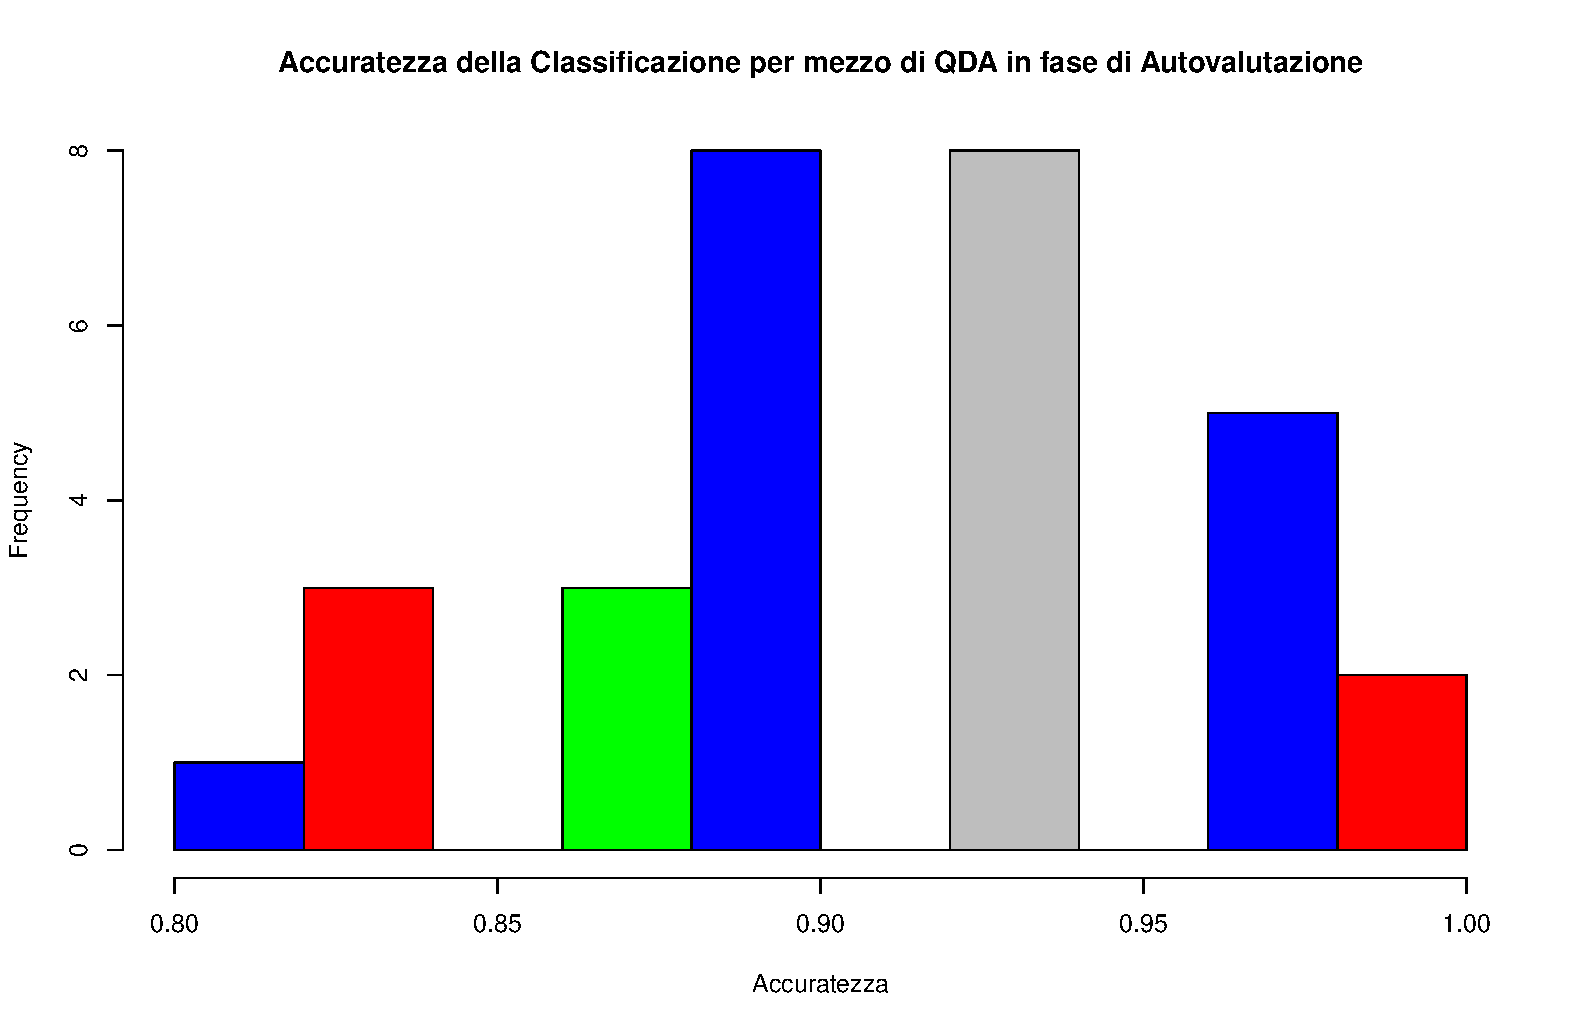
\includegraphics[scale=.6]{imgs/QDA_hist.pdf}
\end{figure}
\subsection{Classificazione per mezzo di Regressione Logistica}
La costruzione di un modello di classificazione per mezzo di regressione
logistica, non trattandosi di una classificazione dicotomica, ha richiesto pi\`u
lavoro, e i risultati ottenuti non sono stati per niente soddisfacenti, tanto da
poter scartare questo modello senza ulteriori approfondimenti. Utilizzando le
stesse $5$ componenti principali si ottiene un'accuratezza di classificazione
pari a circa $69\%$.
\begin{figure}[H]
	\vspace{-1.5cm}
	\hspace{-0.5cm}
	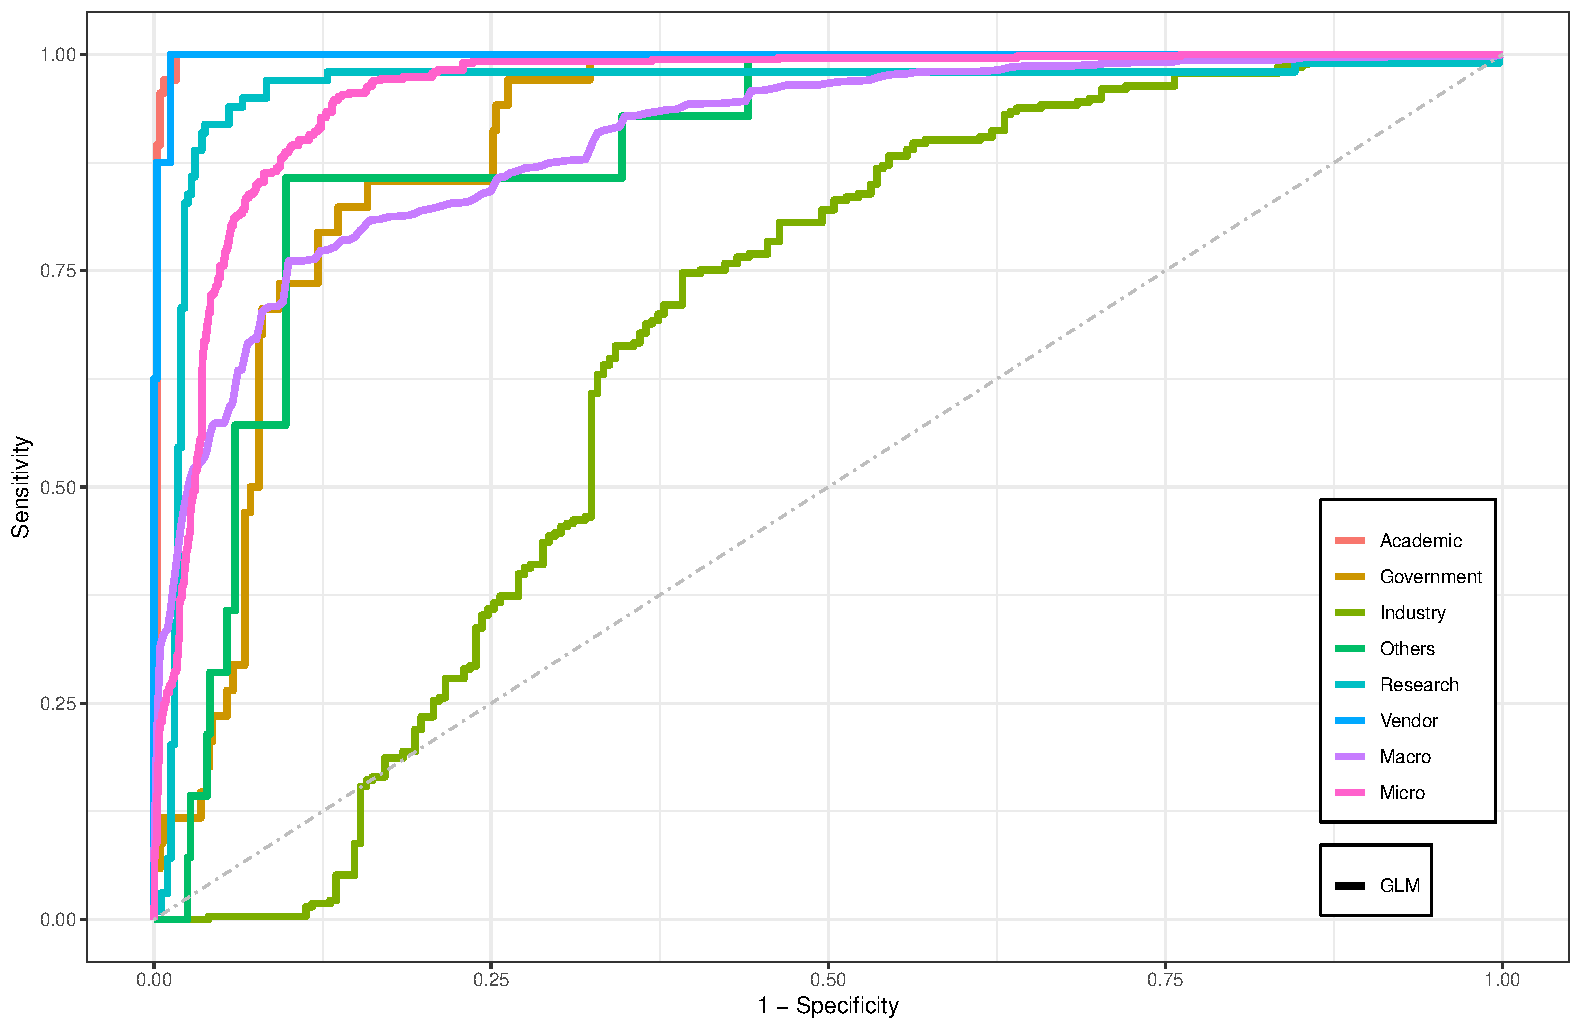
\includegraphics[scale=.60]{imgs/GLM_ggplot.pdf}
\end{figure}

\section{Conclusioni}
In ultima analisi, scartando il modello di classificazione per mezzo regressione
logistica, che fa poco meglio del lancio di una moneta, per quanto riguarda i
due restati modelli presentati, in fase di analisi ho notato che effettuando una
scelta \textit{ad-hoc} delle componenti principali, differente quindi tra LDA e
QDA, si ottiene una capacit\`a predittiva maggiore per entrambi i modelli
superiore al $95\%$. Ottenere questi risultati comporta anche aumentare il
numero di componenti (anche se di poco, uno o due componenti massimo)
principali utilizzate. Per mantenere l'analisi il pi\`u coerente possibile e per
ottenere risultati il pi\`u possibile comparabili, ho utilizzato per tutti i
modelli valutati lo stesso sottoinsieme di componenti principali della PCA.\\
\\
Analizzando con pi\`u attenzione la matrice di confusione dei due modelli, ci
rendiamo conto che entrambi sbagliano nel classificare
\begin{itemize}
	\item osservazioni che fanno parte di classi per le quali si ha un
		elevato numero di campioni;
	\item osservazioni che fanno parte di classi per le quali si ha un
		ridotto numero di campioni;
\end{itemize}
L'interpretazione che ho dato a questo fenomeno \`e che stiamo utilizzando un
numero di fattori molto pi\`u piccolo rispetto a quello originale. Ricordiamoci
infatti che la tabella originale conteneva $37$ colonne e che i modelli che
abbiamo analizzato noi utilizzano solamente $5$ fattori. Evidentemente quindi,
l'errore non \`e dovuto solamente a una scarsit\`a o abbondanza di campioni per
la particolare classe analizzata, ma anche a qualche fattore mancante che
porterebbe certamente ad una maggiore proporzione di varianza spiegata della
struttura delle osservazioni originarie.\\
\\
Notiamo anche che il modello di classificazione per mezzo di LDA e quello per
mezzo di QDA sbagliano in fase di predizione relativamente a classi differenti.
\`E quindi certamente possibile ottenere un modello di classificazione migliore
utilizzando il migliore per ciascuna classe.
\end{document}
